\documentclass[pdftex,12pt,a4paper]{article}
\usepackage{mathptmx}
\usepackage{blindtext}
\usepackage{graphicx}
\usepackage{subfiles}
\usepackage{amsmath}
\usepackage{amsthm}
\usepackage{tikz}
\usepackage{wrapfig}
\usepackage{lscape}
\usepackage{rotating}
\usepackage{epstopdf}
\usepackage{subcaption}
\usepackage[font=small,labelfont=bf]{caption}
\usepackage{hyperref}
\usepackage{color}
\usepackage{algorithm}% http://ctan.org/pkg/algorithms
\usepackage{algpseudocode}% http://ctan.org/pkg/algorithmicx
\hypersetup{
    colorlinks=true,
    linkcolor=blue,
    citecolor=blue
}
\theoremstyle{definition}
\newtheorem{definition}{Definition}[section]
\newtheorem{theorem}{Theorem}[section]
\newtheorem{lemma}[theorem]{Lemma}
\theoremstyle{remark}
\newtheorem*{remark}{Remark}
\usepackage{amssymb}
\usepackage{amsfonts}
\usepackage{mathtools}
\usepackage{geometry}
 \geometry{
 a4paper,
 total={210mm,297mm},
 left=20mm,
 right=20mm,
 top=20mm,
 bottom=20mm,
 }
\renewcommand{\baselinestretch}{2.0}
\newcommand{\defeq}{\vcentcolon=}
\newcommand{\eqdef}{=\vcentcolon}
\newcommand*{\V}[1]{\mathbf{#1}}%
\newcommand{\norm}[1]{\left\lVert#1\right\rVert}
\newcommand{\justif}[2]{&{#1}&\text{#2}}
\newcommand{\qedwhite}{\hfill \ensuremath{\Box}}
\newcommand\given[1][]{\:#1\vert\:}
\newcommand{\me}{\mathrm{e}}
\DeclarePairedDelimiterX{\infdivx}[2]{(}{)}{%
  #1\;\delimsize\|\;#2%
}
\DeclarePairedDelimiter\abs{\lvert}{\rvert}%
\newcommand{\Conv}{\mathop{\scalebox{1.5}{\raisebox{-0.2ex}{$\ast$}}}}%
\newcommand{\infdiv}{\infdivx}
\newcommand\tab[1][1cm]{\hspace*{#1}}
\newcommand{\parder}[2]{\frac{\partial{#1}}{\partial{#2}}}
\renewcommand{\qed}{\hfill\blacksquare}
\hyphenation{op-tical net-works semi-conduc-tor tech-no-lo-gy}



\title{Interpretable Recurrent Neural Network Architectures for Time Series Prediction}
\author{Bernardo P\'erez Orozco}
\date{}
\begin{document}

\maketitle

\begin{abstract}
    The Long Short-Term Memory (LSTM) model is a special case of the more general Recurrent Neural Networks (RNNs) approach. However, RNNs have been known to be difficult to train by means of gradient descent methods because they suffer from the vanishing gradient problem, which prevents them from learning long term dependencies. The LSTM architecture directly tackles this problem by incorporating a gating mechanism that allows training error signals to flow backwards for long periods of time, and hence is able to learn long term relations using gradient-based methods. In this document we summarise some of the most relevant literature for the development of the LSTM Architecture for time series prediction, and give a work plan that addresses some of its weaknesses. 
\end{abstract}

\section{Introduction}

\par The document is structured as follows: in Section \ref{sec_path} we give a refresher on basic Neural Networks concepts, summarise recent upgrades developed for gradient descent methods, and discuss the RNN architecture and the vanishing gradient problem. In Section \ref{sec_lstm} we introduce the LSTM architecture and show how this approach solves the vanishing gradient problem. Then, in Section \ref{sub_future}, we give an account of further thoughts for future work and opportunities for LSTMs in both the research community and industry.

\section{A review of Neural Networks} \label{sec_path}
\subsection{Multilayer Perceptron}
In this section, we give a brief refresher of basic concepts of neural networks. Throughout this document, we will present several architectures that should be thought of as blocks. Connecting these blocks or layers using a specific topology yields what we traditionally call \textit{a neural network}. 

\par A neural network layer contains computing units, also called \textbf{neurons}. Each neuron receives a vector input $\V{x}$ and computes a scalar $h$ called the \textbf{activation} of the neuron \cite{Bishop2006}. The activation value computed by each individual unit describes the amount of activity in the neuron, and hence we can think of them as \textbf{feature detectors} \cite{Touretzky1989}, i.e. certain stimuli (features) will increase the activity of specific units. The vector of activations $\V{h}$ is obtained by gathering the activation values of all individual neurons in a single layer, and it describes the current state of the layer. This vector can then be passed on to other layers in order to make decisions.

\par The simplest case of a neural network is called a Multilayer Perceptron (MLP) and comprises three layers: an input layer, a hidden layer, and an output layer \cite{Bishop2006}. These are connected one after the other, i.e. in a feedforward fashion. The hidden and the output layers are both instances of \textbf{dense layers}. Each neuron in a dense layer is fully connected to all the neurons in the previous layer and its activation is given by $h = \phi(\V{w}^T\V{x} + b)$, where $\V{w}$ is the parameter vector of the neuron, $b$ is the bias parameter of the layer, $\V{x}$ is the input to the layer, and $\phi$ is called the activation function, as seen in Figure \ref{fig:neuron}.

\begin{figure}[h]
    \centering
    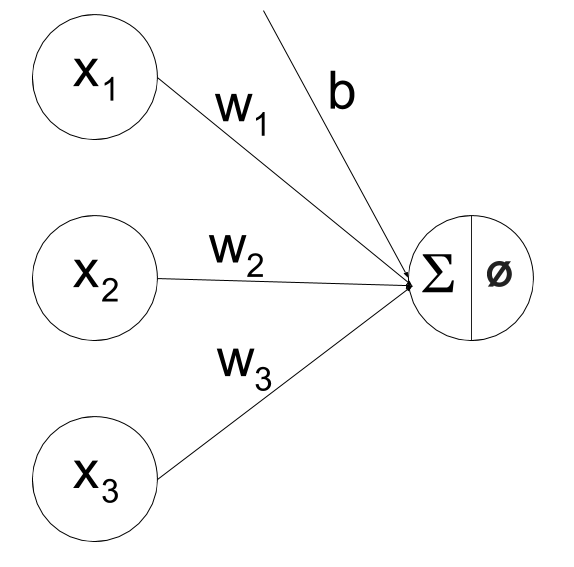
\includegraphics[width=5.5cm]{figs/neuron.png}
    \caption{The dense unit is fully connected to all units in the previous layer. Each edge is weighted by a scalar $w_i$, and the function learnt by the neuron has a vertical shift given by a bias $b$. The activation of the dense unit is given by $h = \phi(\V{w}^T\V{x} + b )$.}
    \label{fig:neuron} 
\end{figure} 

\begin{figure}[h]
    \centering
    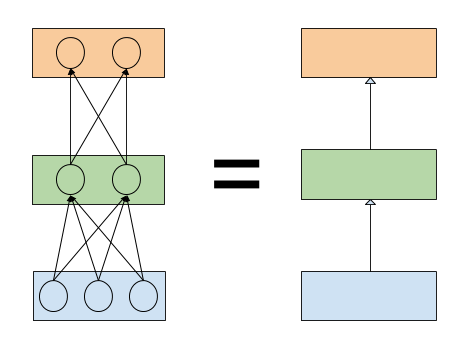
\includegraphics[width=6cm]{figs/mlp.png}
    \caption{Although the processing units of neural networks are its hidden units, the model itself can be thought of as a set of interconnected layers. Each layer can be thought of as a mapping with a specific shape.}
    \label{fig:mlp}
\end{figure}

\par However, neural networks are generally thought of in terms of layers, not individual neurons. We can think of layers more generally as mappings (characterised by some fixed parameters $\theta$) between two spaces, and then a neural network is created by connecting them, as seen in Figure \ref{fig:mlp}. For example, we can think of dense layers as mappings $H:\mathbb{R}^n \rightarrow \mathbb{R}^m$ given by $H(\V{x}) = \phi(\V{Wx}+\V{b})$, where:

\begin{itemize}
    \item The entries of the output vector $\V{h} = H(\V{x})$ are called the \textit{activations} of the layer.
    \item $\phi$ is an element-wise function called the \textit{activation function}.
    \item $m$ is called the \textit{size} of the layer, and refers to its number of \textit{hidden neurons}.
    \item $\theta = \{\V{W, b}\}$ are called the parameters of the layer.
\end{itemize}

\par Activation functions are often called \textit{non-linearities}, since they are expected to be non-linear - some common examples in the literature are the sigmoid activation function, the hyperbolic tangent and the rectified linear unit, given respectively by:
\begin{align*}
    \sigma(x) &= \frac{1}{1+e^{-x}}\\
    \text{tanh}(x) &= \frac{e^x - e^{-x}}{e^x + e^{-x}}\\
    \text{ReLU}(x) &= \max(0, x)
\end{align*}

\par Remark that the usage of non-linearities is crucial for allowing neural networks to learn complex relations in data. Each successive layer will receive as input a vector that will have gone through a non-linear transformation, and therefore neural networks are able to learn very complex, non-linear geometries.

\par It can be shown that an MLP with one hidden layer with a linear activation function can be reduced to an MLP with only an output layer, and hence linear activations are reserved for output layers in problems such as time series prediction, i.e. when we are concerned with unconstrained, continuous output.

\subsection{Deep learning and model selection issues}
\par Deep learning is a subfield of Machine Learning that is concerned with models that have ``a large number of layers''. Deep networks hence are those that satisfy this requirement. In this context, some members of the academic community might consider a 5-layer model to be deep, although a large portion of the most successful deep networks will actually have more than 10 \cite{Szegedy,Simonyan2015}.

\par The development of deep learning has also made available a number of new layers, in particular, the LSTM, the convolutional layer and the autoencoder. Even though in this work we are mainly concerned with the LSTM architecture, there exist several model selection issues that are relevant to the wider neural network academic community, in particular: given a problem, how many and what type of layers should a network have in order to exhibit good performance? How many hidden units and what activation function should each of these layers have? How do we find the optimal values for the parameters $\theta$ so as to maximise the network's performance?

\par All of these model selection issues still represent a priority in the neural network agenda, since there is no single correct answer to any of the questions above. Furthermore, they raise even more questions regarding the effectiveness and interpretability of neural networks, e.g. is the hidden representation learnt by intermediate layers meaningful in any way? Or, for a given problem, is there a problem formulation for which the solution becomes more explicit, i.e. a mathematical relation between the optimal solution and the number of parameters of the network?

\par One further question concerns the effectiveness of deep networks against simpler ones. More specifically, what is the mathematical underpinning that makes deep networks have better performance? One motivation is to learn features automatically in a hierarchical fashion, i.e. assuming that a a sequential application of linear and non-linear transformations would output an optimal feature representation from data, and that an additional dense layer could be used to perform the desired task (regression, classification, etc.). 

\par Although some of these hypotheses were first proposed in the 90s \cite{Hochreiter1997}, the lack of specialised hardware and software disallowed the academic community from bringing these models to life. This is one of the main reasons why, even though it was actually conceived last century, it is only now that we have seen deep learning in practice.

\par One of the most successful deep learning models is the Long Short Term Memory (LSTM) cell, which is a recurrent architecture that enables efficient learning of generic Recurrent Neural Networks (RNNs). In the next subsections, we introduce recurrent networks and training by gradient descent, which naturally leads to a presentation of the LSTM architecture.

\subsection{Recent developments for gradient descent}

Given a neural network with layers $H^{(1)}, H^{(2)}, ..., H^{(L-1)}$, where $L$ is the number of modules in the network, we are now concerned with finding the values of each layer's parameters, e.g. if $H^{(i)}$ is a dense layer, we now want to find the values of $\V{W^{(i)}, b^{(i)}}$ that optimise a \textit{criterion}, also called a \textit{loss function}. The criterion is chosen with respect to the sort of problem to be tackled, and is parametrised by the data's ground truth, for example:

\begin{itemize}
    \item \textbf{Minimum squared error}. Defined as the 2-norm distance between $m$ predictions and the ground truth: $L_\text{MSE}(\hat{\V{y}}) = \frac{1}{m}\norm{\V{\hat{y}} - \V{y}}^2$. This is a common choice for regression problems.
    \item \textbf{Cross-entropy}. For classification problems with $K$ classes, a model can output a probability $y_{nk}$ that an instance $\phi_n$ in the dataset belongs to class $k$. Consider the 1-of-$K$ encoded distribution of the target class $\V{t}_n$. Then, the cross-entropy between the prediction distributions and the target class distributions for a dataset with $N$ samples is given by \cite{Bishop2006}:
    \begin{align*}
        L_{\text{xent}}(\V{y}) = -\sum_{n=1}^N\sum_{k=1}^K\ln t_{nk}{y_{nk}}
    \end{align*}
    
    \item \textbf{Hinge loss}. In classification problems, this margin-based function increases based on the number of misclassifications produced by the algorithm. For the binary case with ground truth and prediction $\hat{y}, y\in\{1, -1\}$, the hinge loss is given by $L_\text{hinge}(\hat{y}) = \max{(0, 1 - \hat{y} \odot y )}$.
\end{itemize}

%cite: http://www.cs.toronto.edu/~graves/icml_2006.pdf
\par The loss function speaks about the fitness of our predictions with respect to the data. This is why bespoke loss functions may be more suitable for specific problems - for example, the Connectionist Temporal Classification loss \cite{Graves2013}, which improves sequence classification by ``removing inherently ambiguous label boundaries and allowing label predictions to be grouped together if it proves useful''.

\par Once a loss function has been chosen, we can use an optimisation method to minimise it. The most widespread method in the neural network community is gradient descent, which finds an optimal solution in an iterative fashion. However, it is worth noting that many alternatives are still being researched, for example evolutionary algorithms \cite{Sexton1999,Schmidhuber2007}, Bayesian optimisation techniques \cite{Bishop1995} and Kalman filters \cite{Tobergte2013}.

\par The simplest variant of gradient descent updates the parameters $\theta$ once per epoch (a single scan of the dataset) using the rule:
\begin{align*}
    \theta_{t+1} = \theta_{t} - \alpha \nabla_\theta L(\theta) 
\end{align*}

where $\alpha$ is called the learning rate and $L$ is the loss function to minimise. Recent developments to this version of gradient descent (and which have seen the light of day on par with the deep learning wave) include:

\begin{itemize}
    \item The advent of big datasets has made a single computation of the true gradient of $L$ too expensive, since a single update operation requires a scan of the whole dataset. \textbf{Minibatch stochastic gradient descent} (minibatch SGD) \cite{Bottou2010} instead computes an approximation of the gradient using only a (random) ``minibatch'' of the dataset. The approximate gradient is computed as the empirical mean of the gradient evaluated at each individual data point in the dataset. As the number of points used to take the empirical mean grows larger, we expect the approximation to converge to the true gradient. This variant of gradient descent is stochastic because the approximate gradient is a random variable subject to the random minibatch - this helps the method escape from local minima if it gets stuck, and also encourages the exploration of a larger area of the loss function (as opposed to the deterministic nature of vanilla gradient descent, which always explores the same area for the same given initial conditions).
    \item The value of the learning rate $\alpha$ hyperparameter can greatly influence the performance of the algorithm. A value too large and the algorithm will struggle to converge. A value too small and the algorithm will take a very long time to finish. Furthermore, some input features may be sparser than others, and thus we would like to take full advantage of their rare occurrences. \textbf{Adaptive Learning Rate} methods aim to solve both of these issues by allowing the learning rate to adapt automatically over time, normally considering information unveiled by previous gradient computations. AdaGrad (Adaptive Gradient) \cite{Duchi2011} was the pioneer in this class of techniques. Let $g_\tau$ be the approximate gradient at time $\tau$, and let $G_i=\sum_{\tau=1}^t g_{\tau, i}^2$. Then the update for the i-th parameter $\theta_i$, using a smoothing factor $\epsilon$ and initial learning rate $\alpha$, is given by:
    \begin{align*}
        \theta_{t+1, i} = \theta_{t, i} - \frac{\alpha}{\sqrt{G_i + \epsilon}}g_{t, i}
    \end{align*}
    \item The descent can gain \textbf{momentum} by allowing new updates to consider previous updates \cite{Sutskever2013}, i.e. if $\theta_{t+1} = \theta_t - \nu_t$, then allow $\nu_t = \gamma\nu_{t-1} + \alpha\nabla_\theta L(\theta)$, where $\gamma$ is called the momentum factor. Therefore the updates are always pulled or corrected by our knowledge of previous gradients. This greatly dampens the effect of very noisy approximations to the true gradient, while also encouraging taking steps in the best direction.
    
\end{itemize}

%http://sebastianruder.com/optimizing-gradient-descent/index.html#stochasticgradientdescent
\par Some recently developed algorithms that implement these improvements are Adadelta, RMSprop and Adam. Although they all have a similar performance \cite{Kingma2014}, Adam is the one that has shown the best empirical results so far. Adam stands for Adaptive Moment Estimation, where moment in this case refers to the bias-corrected estimates of the first- and second-order moments of the gradient. Adam keeps an exponentially decaying sum of gradients that emulates the performance of momentum. The update equations are given below:

\begin{align*}
    \theta_{t+1} &= \theta_t - \frac{\alpha}{\sqrt{\hat{v_t}} + \epsilon}\hat{m_t}\\
    \hat{m_t} &= \frac{1}{1 - \beta_1^t}\beta_1 m_t\\
    \hat{v_t} &= \frac{1}{1 - \beta_2^t}\beta_2 v_t\\
    m_t &= \beta_1m_{t-1} + (1 - \beta_1)g_t\\
    v_t &= \beta_2v_{t-1} + (1 - \beta_2)g_t^2
\end{align*}
 where $\beta_1, \beta_2 \in (0, 1)$ are called the bias-correction hyperparameters.

\par All the gradient descent variants discussed until now require the computation of a gradient (regardless of whether it is exact or approximate). Traditionally, neural networks have benefited from the backpropagation algorithm, which is an efficient way of computing the gradient $\nabla_\theta L(\theta)$. Backpropagation is different to other gradient computation techniques (namely finite differences and symbolic differentiation) in that it takes advantage of the chain rule and the graph structure of the neural network so as to store intermediate results and hence compute derivatives more efficiently. 

\par A more general approach to compute derivatives is \textbf{automatic differentiation} (AD), which allows to evaluate derivatives of functions specified by computer programs \cite{Kingma2014}. In other words, given a program $P$ that computes a function $f(\V{x})$, we can compute its gradient $\nabla_\V{x}f$ by representing the program as a computational graph that can be traversed. This traversal is equivalent to a successive application of the chain rule to each statement in the program $P$, and it generates a new program $P'$ that computes the gradient $\nabla_\V{x} f(\V{x})$.

\par Crucially, AD introduces several advantages with respect to numerical and symbolic differentiation: it does not introduce round-off or approximation errors, unlike finite differences; it returns an efficient way of computing the gradient, unlike symbolic differentiation, which requires additional computational power to perform all appropriate simplifications; and it takes full advantage of intermediate results to compute the derivative of a vector function with respect to each of its inputs efficiently - both numerical and symbolic differentiation require an independent run to take the derivative of the function with respect to each input. AD has further enhanced the interest in the development of gradient descent methods. In fact, it is now a key component in many specialised software frameworks for deep learning, such as Theano \cite{Bergstra2010,Bastien2012}, Torch \cite{Collobert2011} and Tensorflow \cite{tensorflow} implement AD. More details of the AD framework can be found in \cite{Bucker2005ADA}. 

\subsection{Recurrent Neural Networks}
The networks that have been discussed so far contained layers connected sequentially, i.e. in a feedforward fashion. We now turn our attention to networks that are allowed to form a cyclical topology. These models are called \textbf{Recurrent Neural Networks} (RNNs).

\par The simplest RNN is the one that contains a single dense layer connected to itself, i.e. $\V{h}_t = f(\V{h}_{t-1}, \V{x}_t ; \theta)$, where $\V{x}_t$ is the input to the layer at time $t$. This equation is the standard equation of a dynamical system. We can see this relation more clearly by unrolling the network as seen in Figure \ref{fig:rnn}. This means that this architecture enables us to train models over sequences.

\begin{figure}[t]
    \centering
    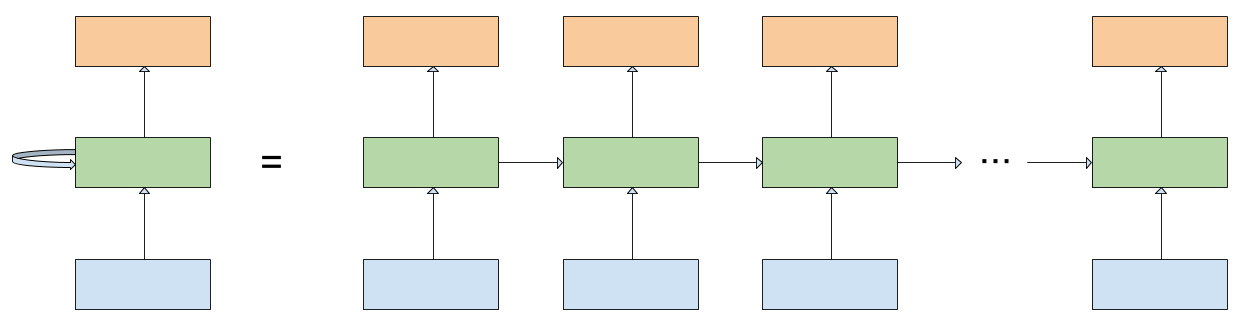
\includegraphics[width=\textwidth]{figs/rnn.png}
    \caption{Recurrent neural networks have at least one directed cycle, often present in the form of a self-connected layer. The resulting graph can be unfolded as a grid, which enables sequence learning to be visualised more clearly.}
    \label{fig:rnn}
\end{figure}

\par The \textbf{RNN layer} is the extension of the dense layer for the recurrent topology, and is given by:
\begin{align*}
    \V{h}_t = \phi(\V{W_rh}_{t-1} + \V{W_ix}_t + \V{b})
\end{align*}

\par i.e. we now have an extra matrix of parameters in comparison with the dense layer. For convenience, we can also define it in the following way:
\begin{align*}
    \V{h}_t = \V{W_r}\phi(\V{h_{t-1}}) + \V{W_ix}_t + \V{b}
\end{align*}

\par From the equation above, it is easy to see that $\V{h}_t = f(\V{h}_{t-1}, \V{x}_t, \theta)$, and furthermore 
\begin{align*}
\V{h}_t = f(f(...f(\V{h}_0, \V{x}_1, \theta)..., \V{x}_{t-1}, \theta), \V{x}_t, \theta)    
\end{align*}
where $\V{h}_0$ is the initial state of the recurrent network. 
\par We are now interested in computing the gradient $\nabla_\theta\V{h}_t$ so as to use gradient descent. A careful derivation of these is given in \cite{Pascanu2012}. However, we will briefly discuss the crucial term $\frac{\partial\V{h}_t}{\partial\theta_j}$, where $\theta_j$ is any parameter in $\theta$. Using the product rule and the chain rule, we can see that:
\begin{align*}
    \frac{\partial\V{h}_t}{\partial\theta_j} &= \frac{\partial\V{W}_r}{\partial\theta_j} \phi(\V{h_{t-1}}) + \V{W}_r\frac{\partial \phi(\V{h}_{t-1})}{\partial\V{h}_{t-1}}\frac{\partial \V{h}_{t-1}}{\partial\theta_j}\\
    &= \frac{\partial\V{W}_r}{\partial\theta_j} \phi(\V{h_{t-1}}) + \V{W}_r\phi'(\V{h}_{t-1})\frac{\partial \V{h}_{t-1}}{\partial\theta_j}\\
    &= \frac{\partial\V{W}_r}{\partial\theta_j} \phi(\V{h_{t-1}}) + \V{W}_r\phi'(\V{h}_{t-1})\left(\frac{\partial\V{W}_r}{\partial\theta_j} \phi(\V{h_{t-2}}) + \V{W}_r\phi'(\V{h}_{t-2})\frac{\partial \V{h}_{t-2}}{\partial\theta_j}\right)
\end{align*}
with $\phi'(\V{h}_{t-1}) = \frac{\partial \phi(\V{h}_{t-1})}{\partial\V{h}_{t-1}}$.
\par We can see that computing $\frac{\partial\V{h}_t}{\partial\theta_j}$ is a recursive process that requires computing $\frac{\partial\V{h}_{t-1}}{\partial\theta_j}, \frac{\partial\V{h}_{t-2}}{\partial\theta_j}, ..., \frac{\partial\V{h}_0}{\partial\theta_j}$, and furthermore each instance of these terms comes alongside another instance of $\phi'(\V{h}_{t-k}), k<t$. This can cause instability, with common activation functions such as tanh and the sigmoid, since their derivatives are never greater than 1 at any location. This is the fundamental disadvantage of Recurrent Neural Networks trained by gradient descent: 
\begin{itemize}
    \item The increasing number of instances of the activation function will lead the gradient to \textbf{vanish}, i.e. a greater number of activation derivative terms is very likely to make the gradient tend to zero.
    \item If the activations are maintained close to 1, but the weights are considerably larger, then adding them up will lead to an \textbf{exploding gradient}. Similarly, this makes it extremely difficult or even impossible (if the gradient overflows the arithmetical precision) for gradient descent to converge.
\end{itemize}

\par In \cite{Pascanu2012}, the authors propose a \textbf{gradient clipping} method to avoid exploding gradients. The authors show how exploding gradient correspond to ``walls'' in the geometry of the loss function. Following the gradient in this case makes the algorithm take a large step away from the wall, and possibly miss the information of the region that lies close by. Instead, the gradient can scaled down whenever it explodes, so as to make the algorithm barely move away from the wall and keep exploring that region. 

\par The clipping rule is given by:
\begin{algorithm}
\begin{algorithmic}[1]
\Function{clip}{$L, \theta, \epsilon_{\text{clip}}$}
\State $\hat{\V{g}} \leftarrow \parder{L}{\theta}$
\If{$\norm{\hat{\V{g}}} \geq \epsilon_{\text{clip}}$}
\State $\norm{\hat{\V{g}}}\leftarrow \frac{\epsilon_{clip}}{\norm{\hat{\V{g}}}}\hat{\V{g}}$
\EndIf
\EndFunction
\end{algorithmic}
\end{algorithm}

\par On the other hand, the most successful attempt so far to tackle the vanishing gradient problem consists in making changes to the recurrent architecture's components. This resulted in the creation of the \textbf{LSTM layer}, which we are now prepared to discuss in the next Section.

\section{The LSTM architecture} \label{sec_lstm}

We now turn our attention to the LSTM architecture. In subsection \ref{sub_lstm}, we will introduce the LSTM cell and show how it solves the vanishing gradient problem. Then, in subsection \ref{sub_apps} we briefly list some of the most recent successful applications of LSTMs.

\subsection{The LSTM cell solves the vanishing gradient problem} \label{sub_lstm}
The LSTM layer \cite{Hochreiter1997,Gers2002} directly addresses the issue of the vanishing gradient by means of a gating mechanism, and is given by the following equations\footnote{The notation $\V{y}\odot \V{z}$ is the element-wise product of the vectors $\V{y,z}$.}:

\begin{align*}
    \V{x}'_t &= [ \V{x}_t, \V{h}_{t-1} ]\\
    \V{S}_t &= \tanh(\V{W}_S\V{x}'_t + \V{b}_S)\\
    \V{C}_t &= \V{i}_t\odot\V{S}_t + \V{f}_t\odot\V{C}_{t-1}\\
    \V{h}_t &= \V{o}_t \odot \tanh(\V{C}_t)
\end{align*}
\par where $\V{i}_t, \V{o}_t, \V{f}_t$ are called the input, output and forget gates respectively, and are given by:
\begin{align*}
    \V{i}_t &= \sigma(\V{W}_i\V{x}'_t + \V{b}_i)\\
    \V{o}_t &= \sigma(\V{W}_o\V{x}'_t + \V{b}_o)\\
    \V{f}_t &= \sigma(\V{W}_f\V{x}'_t + \V{b}_f)
\end{align*}

\par We call $\V{C}_t$ the \textit{memory cell} at time $t$, and it is arguably the main component of the LSTM architecture. It simulates a computer READ and WRITE operations over its memory. For example, we can think of the memory cell equation given above as follows:

\begin{align*}
    \V{C}_t &= \V{i}_t\odot\V{S}_t + \V{f}_t\odot\V{C}_{t-1}\\
    \text{memory}_t &= \text{read}\odot\text{input}_t + \text{remember}\odot\text{memory}_{t-1}
\end{align*}

\par Crucially, the LSTM architecture is based on a \textbf{Constant Error Carousel} (CEC). When thinking of the network as an unfolded computational graph, backpropagation allows the error signal to flow backwards across the nodes. However, a vanishing gradient architecture will dampen the signal as it traverses the graph by a factor given by the derivatives of the activation function. 

\par In other words, we need to stabilise the products $\V{W}_r\phi'{(\V{h})}$ by making them approach $\V{1}$. One way to do this is to regularise the weights while also using a linear activation function for the recurrent edges.  The LSTM layer manages to address this by introducing specialised gates that control the state of each memory cell by regulating the influx of its two main sources: the input at time $t$ and the storage at time $t-1$. Importantly, the behaviour of the gates is also a learning target since we introduce new parameters $\V{W}_i, \V{W}_o, \V{W}_f$ correspondingly.  

\par Note that the memory cell $\V{C}_t$ is only squashed in the feedforward arrows of the networks, and remarkably not in the recurrent computations, i.e. $\V{C}_t$ is a function of $\V{C}_{t-1}$ without any activation. To observe this more formally, we can make a derivation similar to the one for the RNN layer:

\begin{align*}
    \parder{\V{h}_t}{\theta_j} &= \parder{\V{o}_t}{\theta_j}\odot \tanh(\V{C}_t) + \V{o}_t\odot\parder{\tanh(\V{C}_t)}{\V{C}_t}\parder{\V{C}_t}{\theta_j}\\
    \parder{\V{C}_t}{\theta_j} &= \parder{\V{i}_t}{\theta_j}\odot\V{S}_t +  \V{i}_t\odot\parder{\V{S}_t}{\theta_j} + \parder{\V{f}_t}{\theta_j}\odot\V{C}_{t-1} + \V{f}_t\odot\parder{\V{C}_{t-1}}{\theta_j}
\end{align*}

\par By using a similar reasoning to the previous derivation, we can see that the factors $\parder{\V{i}_t}{\theta_j}, \parder{\V{o}_t}{\theta_j}, \parder{\V{f}_t}{\theta_j}, \parder{\V{S}_t}{\theta_j}$ may all (partially) vanish, since they are recursive (dependent on $\V{x}'_t$) and have the shape $\phi(\V{Wx}'_t + \V{b})$. 

\par Nevertheless, the term $\parder{\V{C}_t}{\theta_j}$ is also a function of $\parder{\V{C}_{t-1}}{\theta_j}$, which is different in two ways: firstly, the recursive factor $\V{C}_{t-1}$ is not squashed by any activation function. Secondly, each recursive term is weighted by the element-wise product of the previous $k$ forget gates $\prod_{T=k}^t\V{f}_T$. Therefore, the gradient only vanishes for terms that contain $\V{f}_k$ starts decreasing, and hence the LSTM is allowed to store values in the long term.

\par However, note that the usage of gates does not prevent an exploding gradient from appearing. In fact, the prolonged accumulation due to a forget gate that never turns off can be an additional cause leading to an exploding gradient. This is why LSTMs too are often equipped with gradient clipping.

\subsection{LSTM applications} \label{sub_apps}
LSTMs are state-of-the-art models for sequence learning. As such, they have greatly contributed to the deep learning wave by being applied in several domains. Some examples are: speech recognition \cite{Graves2013}, handwriting generation \cite{Graves2013_2}, financial forecasting \cite{Rutkauskas2011}, machine translation \cite{Sutskever2014}, reinforcement learning \cite{Hausknecht2015} and models of attention (scene labelling) \cite{You2016,Long2014}. 

\par It is important to consider that most of the above are classification problems at different scales, since they consist in assigning phonemes, image categories, words or actions to an input sequence. This sheds light on a potential opportunity: can LSTMs also become a state-of-the-art model for time series forecasting?

\section{LSTMs: challenges and future work} \label{sub_future}
In this section, we first outline some of the challenges that have been identified for LSTMs, and then propose a plan on the short, medium and long term.

\subsection{Challenges and opportunities}
Like many of the other deep learning models, LSTMs have set new records on many Machine Learning tasks, and have become a widespread tool running mobile phones and tablets. However, there are still plenty of areas of opportunity, which we outline below.

\par Firstly, LSTMs are not endowed with any sort of \textbf{probabilistic reasoning}. In particular, LSTMs do not have a direct means of computing prediction errors, contrary to other state-of-the-art models such as Gaussian Processes. Allowing for this is crucial in prediction tasks, specially if they are safety-critical. In the paper accompanying this document we have shown a way to compute these error bars, albeit it requires a vast amount of resources. Additionally, it does not carefully choose what models to take into account, and thus the error bars contain models that do not necessarily contribute for a better explanation of the data.

\par Secondly, neural networks in general suffer from a lack of \textbf{interpretability} due to their black box nature. Although there is some work on the visualisation of LSTMs for specific problems, such as \cite{Karpathy2016}, a formal and general enough framework that allows for the deep understanding of inner dynamics and latent representations learnt by LSTMs is still missing. For example, Principal Component Analysis returns a decorrelated representation of the data, just like Independent Component Analysis learns a representation based on independent sources. Is there any such way of interpreting the hidden, time-ordered representations represented in LSTMs?

\par Thirdly, most LSTM applications tackle classification problems (such as speech recognition). Only a handful of them directly addresses the problem of \textbf{forecasting} real-valued time series. Time series forecasting is one of the biggest problems in science and industry, since it is present in very relevant applications such as weather forecasting, stock market prediction, chaotic series and differential equations analysis, astrophysics and environment quantification, to mention a few. Evaluating whether LSTMs can contribute to the state of the art of any or all of these problems is therefore one of the top tasks in the LSTM research agenda.

\par Fourthly, from a mathematical perspective it still isn't entirely clear what is the effect of certain \textbf{model selection issues}, such as adding or removing layers from a neural network or choosing the number of neurons in each layer. From the accompanying paper though we can see that there seems to be a relation between the confidence of a neural network's prediction and its number of layers. This suggests that a more formal and rigorous explanation can still be found.

\par Fifthly, from the accompanying paper we can also see that the effect of classical \textbf{regularisation} techniques, such as $L_2$-regularisation, do not seem to have a major effect in LSTMs. More recent developments such as Dropout have also been investigated \cite{Srivastava2014}, but the issue of how to regularise LSTMs optimally still remains open.

\par Sixthly, finding a single LSTM with low generalisation error, even with a fixed topology, still relies on having luck when initialising gradient descent. In some of the accompanying paper's experiments, we found that trained LSTMs may not generalise well and instead get stuck in a constant state that makes them predict the same sample over and over again, as seen in Figure \ref{fig:decay}. The very existence of LSTMs is a response to the weaknesses of this optimisation method. Therefore it also makes sense to ask if different \textbf{optimisation methods} would allow plain RNNs to become state-of-the-art. One such attempt is presented in \cite{Schmidhuber2007}, where an RNN is trained using an evolutionary optimisation algorithm and then beats LSTM in sinewave forecasting.

\begin{figure}[t]
    \centering
    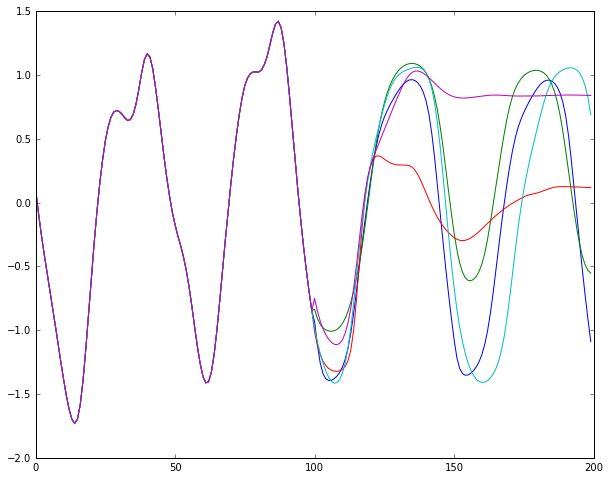
\includegraphics[width=8.5cm]{figs/decay.png}
    \caption{Five prediction sequences generated by different LSTMs using the same seed. The first 100 samples correspond to the seed, and the last 100 are the predicted samples. Two of the predicted sequences stop following the series' trend after the first 30 samples approximately.}
    \label{fig:decay} 
\end{figure} 

\par In conclusion, there are still many open issues that can be tackled in order to make LSTMs be a more robust and interpretable model. These are all crucial features of desirable models, since they enable the introduction of human reasoning while also giving better guarantees with respect to the performance of the model. 

\subsection{Proposal}
From the challenges outlined above, we can see that neural networks need to incorporate a more rigorous mathematical framework. For example, model selection is still done in a brute force fashion, and this is partially due to the lack of interpretability of models. This puts them in disadvantage in comparison with other state-of-the-art models, such as Gaussian Processes (GPs), in which the model's hyperparameters are interpretable and therefore model selection can be done in a rigorous manner \cite{Rasmussen2006}.

\par Another important omission in the literature is the application of LSTMs in forecasting problems. In order to succeed in this domain, LSTMs would still have to prove their capabilities against other models (namely GPs) for two reasons: on one hand, even with a fixed topology, several runs of gradient descent might be needed in order to find a single LSTM that generalises well; on the other hand, even with one such LSTM, several more runs may be required in order to give approximate error bars to our prediction - unlike GPs, which naturally account for them.

\par As a consequence, the current proposal for the remaining portion of my doctorate is focused on these two axes: on one side, developing a more interpretable and mathematically-grounded framework for LSTMs and other recurrent architectures model selection; on the other, improving the performance of LSTMs for time series prediction, which in this context means not only making them forecast more accurately, but also endowing them with the capability of reasoning probabilistically and crucially, producing error bars for their own predictions. 

\subsubsection{Goals in the short term}
In the short term, I will be tackling the first axis described above. In particular, I will be addressing the effect that the number of neurons and layers in a neural network topology have in the predictive likelihood distribution of the model. 

\par One way to measure the predictive likelihood distribution of LSTMs is the one proposed in the accompanying paper, in which we train several LSTMs by initialising the gradient descent method at different locations and then measure the statistics of the resulting distribution. Two of the disadvantages of this method are its low speed and the fact that several runs may take too long before reaching a local minimum. For small datasets, one way to improve this method is by experimenting with different optimisation procedures from the literature: for example, natural gradient methods \cite{Pascanu2014} and Hessian-free optimisation \cite{Martens2010}, or Variational Bayes methods in order to approximate the predictive distribution \cite{Snelson2005}. These results will also shed light on model selection and interpretability issues, since they will give a clearer idea of what the governing rules behind the number of neurons and layers are. 

\par Another interpretability issue that we have started investigating concerns the optimality of hidden representations learnt by neural networks. In Figure \ref{fig:inter} we show the evolution through of the internal state of an LSTM layer that has been trained in the Mackey Glass dataset (as presented in the accompanying paper). Each row represents the state of a single neuron in the layer, and it turns red as its activity increases. It can be seen that each neuron is quasi-periodic, which suggests that they are learning to detect features with a fixed periodicity in our data. One goal in this project is thus to investigate what these features are and how they change as the model settings (number of layers and neurons) change.

\begin{figure}[t]
    \centering
    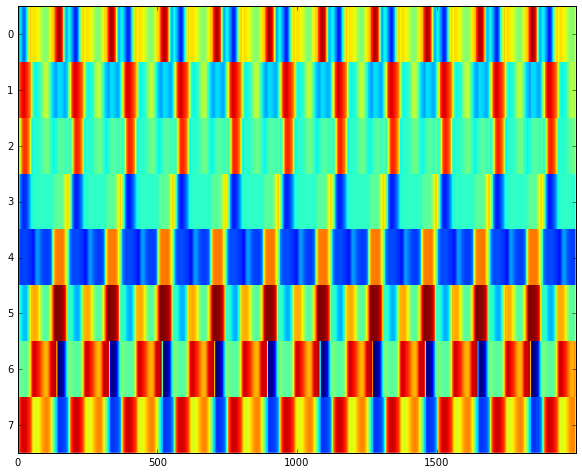
\includegraphics[width=8.5cm]{figs/inter.png}
    \caption{Evolution through time of the internal state of an LSTM for the Mackey Glass time series. Each row represents the amount of activity in a neuron, where red means greater activity, i.e. the presence of a feature. }
    \label{fig:inter} 
\end{figure} 

\par In the upcoming year, the two projects above should end in two deliverable papers to big conferences in Machine Learning. Important submission deadlines to this end are: ICML 2017: Feb 5th 2017 and NIPS 2017: May 2017.

\subsubsection{Goals in the mid-to-long term}
In the mid-to-long term, one of my goals is to use the results obtained in the previous phase in applied settings. Two examples are acoustic signal synthesis and financial datasets. In both cases, having interpretability and model selection at hand will allow to bring in concepts from other domains of knowledge that can improve performance.

\par Earlier this year, we started investigating birdsong synthesis with LSTMs and encountered several challenges. One of them concerns the birdsong feature representation to be fed into the LSTM. Whereas there are plenty of options from the speech recognition literature, such as Mel-frequency Cepstral Coefficients (MFCCs) and Linear Prediction Coefficients (LPC) \cite{Jurafsky2009}, most of these are either non-invertible or lossy. However, one of the main promises of deep learning is also the ability to be able to learn optimal feature extraction independently. In this long-term project proposal, I propose to develop a neural network architecture that is able to extract features from the full Fourier frequency spectrum of a signal, and then learn to synthesise new signals. 

\par Another problem that we observed in this preliminary experiments is a high-dimensional version of the problem we presented in Figure \ref{fig:decay}. By training an LSTM on different representations of birdsong signals and then attempting to predict future samples, the LSTM would quickly reach a constant state and stop producing new samples. This project is a long term goal in which I aim to incorporate the knowledge that will gathered in the first phase regarding model selection so as to build an architecture that incorporates knowledge from the Signal Analysis domain so as to avoid these issues.

\par In the case of financial datasets, it is critical to have models that can be confident about their predictions (or speak about their lack of knowledge). In this case, we are interested in endowing LSTMs with the ability to produce error bars around their predictions. In the accompanying paper, we have proposed a method that does this job, but in an expensive manner, since it samples LSTMs by repeatedly training by gradient descent. In this project, we will use the results obtained in the first phase regarding the optimisation of neural networks in order to endow neural networks with probabilistic reasoning more efficiently.

\par By the end of the next 2-2.5 years, I aim to incorporate the projects outlined above into a single thesis whose main contribution is a substantial improvement to the neural network model selection and interpretability literature, and show their applications in finance and acoustic signal synthesis.

\addcontentsline{toc}{section}{Bibliography}
\bibliographystyle{unsrt}
\bibliography{bib}

\end{document}